\chapter{Finite State Machines}

In Chapter 5 the exploration began with sequential circuits, circuits
whose output is a function of the input and current state, and by examining
the basic memory elements. Now, utilization of these basic
memory elements to build general sequential circuit is considered.

The sequential design process starts the same as the combination design
process, with a word statement.  From this word statement, a state diagram is created. 
The logic to control the transitions between the
states is derived directly from
the state diagram.  In cases where the finite state machine (FSM) controls a 
complex system, it may be necessary to build a control word table to 
determine the output equations.  Otherwise, the output equations are derived
directly from the state diagram.  In order to make this discussion more 
concrete, all the FSMs to be designed in this chapter have the 
structure shown in Figure~\ref{fig:GenFSM}.

\begin{figure}[ht]
\center{\scalebox{1.0}{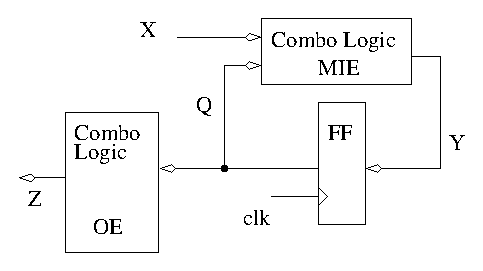
\includegraphics{./Fig7/GenFSM}}}
\caption{The standard structure of a FSM for the current chapter.}
\label{fig:GenFSM}
\end{figure}
\label{page:GenFSM}

Each of the signals $X,Y,Q,Z$ is a vector, consisting of zero or more bits.  
The $X$ signal is the input to the FSM from the system being controlled.  
The $Z$ signal is the output from the FSM to the system being controlled.
The combinational logic circuit generating $Z$ is called the {\it output 
equations} (OE).  The state of the FSM is carried on the $Q$ 
lines.  Each bit of $Q$ is the output of a D flip flop. Thus, if $Q$ is
six bits wide, then the FSM has six D flip flops.  The $Y$ signals are 
called the 
memory inputs; they are the data inputs to the D flip flops.  The combinational
logic circuit generating the $Y$ signals is called the {\it memory input
equations} (MIEs). In order to improve the readability of circuit 
diagrams, from now on, the clock signal will not be shown.
With respect to Figure~\ref{fig:GenFSM}, the design 
of a FSM requires three questions be answered: What are the MIEs; what 
are the OEs; and how many D flip flops are required?  These questions are  
answered by first understanding how to convert a word statement into a state
diagram.


\section{Word Statement to State Diagram}

Since the design of a FSM starts with the conversion of a word statement into
a state diagram, it is imperative to understand what information is captured
in the states of a state diagram.

The states of a FSM can be thought of as the history of previous 
inputs, the operating modes of a system, or the steps in a process.

A state can be used to capture the history of previous inputs.  For example, 
consider a FSM controlling a vending machine which dispenses 
35\textcent sodas.  The
FSM has two bits of inputs, N and D which equal 1 when a nickel or dime is 
inserted.  It has one bit of output which equals when to dispense a soda.  The
states in this FSM would represent how much money has been deposited so far.

A state can be used to capture the operating mode of a system.  For example,
the FSM which controls a furnace in a house might have two states;
on or off.

A state can be used to capture which step a process is in.  For example, 
consider a FSM which controls the movement of milking cows through a chute
in order to read their ID tags.  The FSM has two inputs, one which detects 
if a cow is present in the chute and the other if the ID tag has been
read correctly. The FSM has two outputs, each controlling the position of either
the entrance or exit gates.  The FSM has states such as CowPresent,
WaitToConfirmRead, WaitForCowToLeave, etc..

Regardless of what the states represent, the state diagram must be drawn in the 
same standardized way.  Each state name is drawn inside a circle.  
One of the states is selected to be the state the FSM starts in when 
first powered-up.  This state, referred to as the reset state, is 
denoted by putting an asterisk inside its 
circle.  The FSM is in exactly one state at a given time.  When the clock edge 
arrives, the FSM samples its inputs and transitions to a next state.  Outgoing
arcs from the state are labeled with the input condition which elicits the
corresponding transition.  As mentioned in Chapter 5, the collection of 
outgoing arcs from a state should be complete and unequivocal.  Complete means
that every possible combination of the variables used on the outgoing arcs has 
been described.  Unequivocal means  no ambiguity in the decision of 
the next state exists.

%%----------------State Diagram to Circuit Diagram------------

\section{Design Using Ones Hot Encoding}

In order to transform an abstract state diagram into a real circuit, the 
symbolic state names in the state diagram must be given some binary encoding.  
When the FSM is in a particular state, $S$, the binary coding for $S$ 
is present on the outputs of the flip flops; $Q$ in Figure~\ref{fig:GenFSM}.
Many different ways can be proposed to choose the encoding of states.  The two most 
popular are dense and one-hot.

A dense encoding minimizes the number of bits used to encode the 
states.  This approach 
is a reasonable goal as minimizing the number of bits to encode the states
has the effect of minimizing the number of flip flops in the FSM.  According to
the arguments made on page~\pageref{page:two-to-N}, if a state diagram has $N$ 
states, then each can be assigned a unique binary code using $log_2(N)$ bits.  
For example, if the vending machine state diagram mentioned earlier had eight  
states, then its FSM designed using a dense encoding of states requires 
three bits.  These three bits could be arranged in eight different ways, each representing
one of the states.  Consequently, its FSM would have three flip flops.

A one-hot encoding assigns one flip flop to each state.  When the FSM is in
state $S$, the flip flop associated with state $S$ outputs 1. Since a FSM can
only be in one state at a time, exactly one flip flop in a one-hot encoded FSM 
outputs 1 and all the others output 0.  The name ``one-hot" refers to the 
fact that one of the flip flop outputs is ``hot" or at a logic 1.

Each encoding technique has its own strength and weakness which should 
influence the choice of which to use.  The strength of the dense encoding 
is it minimizes the number of flip flops in the design.  The biggest 
draw-back of using a dense
encoding is it requires a significant effort to minimize the circuits
in the MIEs and OEs. The strength of the one-hot encoding is the fact that
the process of determining the MIEs and OEs is quick and simple.  Furthermore, 
when compared to a dense encoding, the MIEs and OEs of a one-hot encoded FSM
generally require far less logic.
The weakness of the one-hot encoding is it requires far more flip flops
than the dense encoding.

The choice of which encoding boils down to deciding the medium to
use to implement the digital circuit.  Field programmable gate arrays (FPGAs) 
contain a large number of 
standard cells which can be configured and interconnected in a variety of ways.
A one-hot encoding makes sense for FPGAs because the automated design tools 
would have a difficult time optimizing a dense encoding and there is an 
abundance of flip flops available.  In a custom-designed VLSI chip, it would 
make sense to utilize a dense encoding in order to minimize the number of 
gates in the implementation, and hence, the size of the resulting circuit.  
Given the prevalence of FPGAs, 
one-hot encoding is the focus for the states of the chapter's FSMs.

Three steps transform a state diagram into a 
circuit diagram when using a one-hot encoding of the states.  First, 
determine the number of flip flops.  Second, determine the MIEs.
Third, determine the OEs.

The first step is easy; assign one flip flop to each state.  For
each state $S$, label the input of the flip flop $D_S$ and the
output of the flip flop $Q_S$.

The second step requires the derivation of the MIEs.  Since each state
gets its own flip flop and there is one MIE for each flip flop, then there 
is one MIE for each state.  The  MIE for state $S$ should output 1 when the 
FSM transitions to state $S$ in the next clock cycle.  In other words, 
the MIE for state $S$ is the answer to the question, ``How does the FSM get 
into state $S$?"  State $S$ is entered by starting at some state $P$ and 
meeting the condition $c$ on its arc leading to state $S$.  The transition
arc contributes a term $P*c$ to the MIE for state $S$.  If  more 
than one arc terminates at state $S$, then the MIE for $S$ is the logical
OR of the terms from each arc.

For example, in the state diagram shown in Figure~\ref{fig:ones}, three 
arcs terminate at state $S$.  Consequently, the MIE for state $S$ 
consists of three terms, one from each of the arcs.  The arc from state $A$
contributes the term $Q_Ax'y$, the arc from state $B$ contributes $Q_Bx'$,
and the arc from state $C$ contributes $Q_C(x+y')$.  Putting all these terms
together yields the memory input equation $D_S = Q_Ax'y + Q_Bx' + Q_C(x+y')$.

\begin{figure}[ht]
\center{\scalebox{0.8}{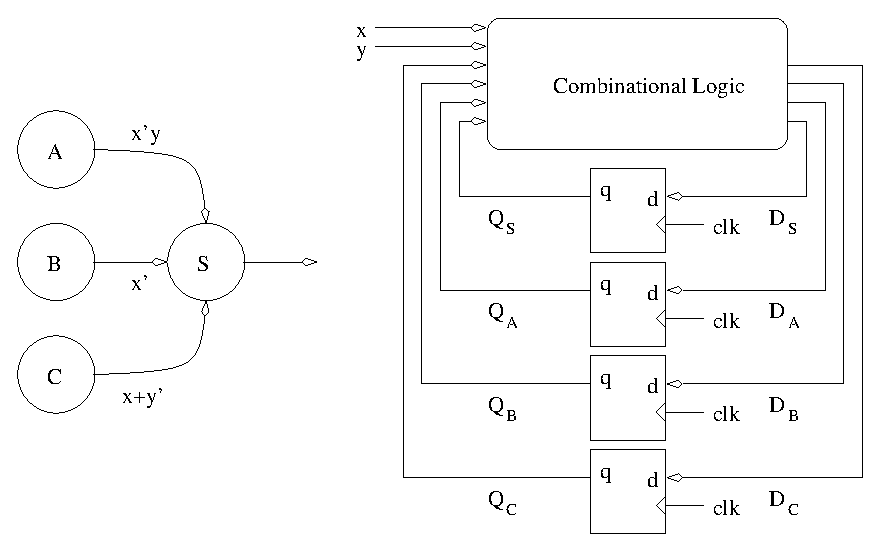
\includegraphics{./Fig7/Ones}}}
\caption{A state diagram and its FSM.}
\label{fig:ones}
\end{figure}

The third step in the transformation of a state diagram into a circuit
diagram requires the elaboration of the output bits and the definition of their
value for each state forming an output table.  From Figure~\ref{fig:GenFSM}, 
see that the OEs are dependent only on the state.  Remember the
output from the flip flop associated with $S$, $Q_S$, equals 1 when the 
FSM is in state $S$.  Consequently, if an output $Z$ equals 1 when the 
FSM is in state $S$, then the output equation for $Z$ will contain the
term $Q_S$.  Consulting the output table for a FSM reveals a list
of states for which an output $Z$ equals 1.  Since the output equals
1 when the FSM is in any of these states, the output equation for $Z$
is the logical OR of these states.

The furnace controller circuit first introduced in Chapter 5 is 
revisited to better understand the concepts illustrated in 
Figure~\ref{fig:ones}.


%%----------------FURNACE CONTROLLER------------

\paragraph{Word Statement} 
Design a FSM which controls a furnace in order to regulate the 
temperature in a house.  The FSM has two bits of input from thermometer,
$T_{hi}$ and $T_{low}$.  When the temperature inside the house 
is greater than the high threshold, then $T_{hi}$ outputs 1; otherwise 
it outputs 0.  When the temperature inside the house is greater than 
the low threshold, then $T_{low}$ outputs 1; otherwise it outputs 0.  
The output from the FSM controls a furnace.  When the FSM outputs a 
1, the furnace turns on, warming the house.  When the FSM outputs a 0, 
the furnace is turned off, causing the house to cool down.  A graph
of this controller's behavior is given in Figure~\ref{fig:HysteresisGraph}.

\paragraph{State Diagram}
The FSM has two bits of input and one bit of
output. The state diagram, shown in Figure~\ref{fig:FurnaceSD}, has
an asterisk in the state {\bf OFF} implying that this state is the reset state. 
Hence, for start-up, the furnace controller is set in the {\bf OFF}
state.

\begin{figure}[ht]
\center{
\includegraphics{./Fig7/FurnaceSD}}
\caption{A state diagram describing the furnace controller.}
\label{fig:FurnaceSD}
\end{figure}

\paragraph{Circuit Diagram}
The circuit for the FSM shown in Figure~\ref{fig:FurnaceSD} requires 
two flip flops because it has two states.  These flip flops can be called
ON and OFF, their inputs $D_{on}$ and $D_{off}$, and their outputs
$Q_{on}$ and $Q_{off}$.

The MIEs are derived directly from the state diagram.  Two arcs
terminate at the {\bf ON} state, thus the MIE for this state  has
two terms, $D_{on} = Q_{off}*T_{low}' + Q_{on}*T_{hi}'$.  Likewise, the
MIE for the {\bf OFF} state has two terms, 
$D_{off} = Q_{on}*T_{hi} + Q_{off}*T_{low}$.

In order to determine the OEs, an output table is constructed.  The 
table is organized by listing each output as a column and each state as a row.
In the case of the furnace controller, this construction is quite simple.
\\ \\
\begin{tabular}{c||c}

State		& Furnace	\\ \hline 
		& 0 off		\\ \hline 
		& 1 on		\\ \hline \hline
ON		& 1		\\ \hline 
OFF		& 0		\\ 

\end{tabular}
\\ \\
Since the single output equals 1 when the FSM is in the {\bf ON} state, 
$Z_{furnace} = Q_{on}$.
Putting all this together yields the complete circuit diagram for the furnace 
controller FSM as shown in Figure~\ref{fig:FurnaceCircuit}.

\begin{figure}[ht]

\center{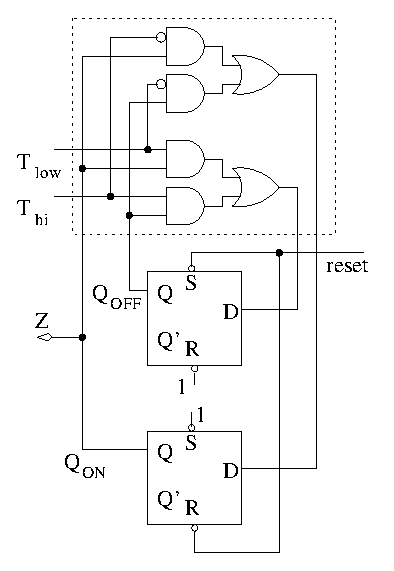
\includegraphics{./Fig7/FurnaceCir}}
\caption{The circuit diagram for the furnace controller.}
\label{fig:FurnaceCircuit}

\end{figure}

One final note needs to be made about the circuit diagram in 
Figure~\ref{fig:FurnaceCircuit}; its reset configuration.  According
to the state diagram shown in Figure~\ref{fig:FurnaceSD}, the
{\bf OFF} state is the reset state.  Hence, the reset signal
is wired to the asynchronous active low set input of the 
OFF D flip flop so that its output goes to logic 1 when the
reset is activated.  All the other flip flops are 
connected to the reset signal through their asynchronous
active low reset input so that their outputs all go to logic
0 on a reset event.

Since the furnace controller operates through time on real
inputs its behavior is better understood in light of applying 
inputs and examining the outputs in a timing diagram.

%%----------------TIMING------------

\section{Design Using Dense Encoding}
\pagebreak
.
\pagebreak
.
\pagebreak
.
\pagebreak
.
\pagebreak
.

\section{Mealy Machines and Moore Machines}
\pagebreak
.
\pagebreak
.
\pagebreak
.
\pagebreak
.

\section{Timing}
Once the FSM is realized, the only way to inspect the behavior of a physical
realization is by applying inputs and observing outputs.  A timing 
diagram is used to examine a sequence of inputs and the resulting behavior of the FSM.
The timing diagram is compared to the state diagram of the FSM in order 
to verify that it is operating as originally designed.  Before diving into an 
example timing diagram,  the sequence of events
occurring  inside the FSM needs to be understood.

The events occurring in the FSM are referenced to the clock input of the 
D flip flops inside the FSM; see Figure~\ref{fig:GenTime}.  Since flip
flops sample their inputs on the positive edge of the clock, this point is the
beginning of the timing analysis, denoted as Event 1 in 
Figure~\ref{fig:GenTime}.  The propagation delay of the flip flops means 
a small delay occurs between the clock edge and the flip flop outputs, $Q$,
becoming valid, Event 2 in Figure~\ref{fig:GenTime}.  The propagation delay 
of the flip flops is denoted $T_{FF}$.  In order to maximize the clocking 
frequency of the FSM, the new inputs, $X$, to the FSM should be applied at the
same moment that the flip flop outputs are becoming valid.  This event is Event 3
in Figure~\ref{fig:GenTime}. According to Figure~\ref{fig:GenFSM}, changing
$Q$ and $X$ has two effects, the outputs $Z$ change and the memory
inputs $Y$ change.  The delay between the application of the new inputs to
the MIE logic and $Y$ is the propagation delay of the combination logic, denoted
$T_{combo}$ in Figure~\ref{fig:GenTime}.  Event 4 denotes the instant in time
when $Y$ becomes valid.  When the $Y$ values are valid, a small
delay occurs while the flip flops register their new inputs, denoted $T_{su}$.  After 
this setup time, the FSM is ready for another clock edge.  

\begin{figure}[ht]

\center{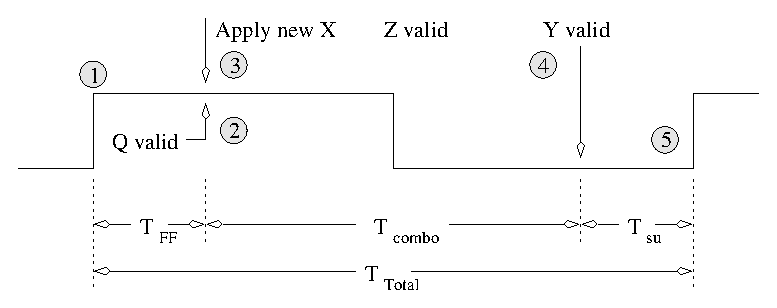
\includegraphics{./Fig7/GenTime}}
\caption{A timing diagram showing the sequence of events in a FSM.
The circled numbers refer to the sequence of events in a FSM.}
\label{fig:GenTime}

\end{figure}
\label{page:GenTime}
\index{timing!FSM}

The total time between the clock rising and the FSM being ready for another 
clock edge, $T_{total} = T_{FF} + T_{combo} + T_{su}$,  is the minimal 
amount of time between successive clock edges.  If a clock edge arrived 
sooner than $T_{total}$, then at the very least, the setup time of the 
flip flops would be violated.  The maximum clocking frequency 
of a FSM is $F_{max} = 1/T_{total}$.

Consider the operation of the furnace controller through time.
To do this, consult the memory input equations of the
FSM in Figure~\ref{fig:FurnaceCircuit}.  A timing diagram, Figure~\ref{fig:FurnaceTime}, 
shows a sequence of inputs applied and the
behavior of the circuit. At some time before time=0, the reset signal is
asserted to logic 0.  This reset event causes the FSM to go into the 
{\bf OFF} state.  The 
reset signal is released prior to time=0, but the FSM stays in the {\bf OFF}
state because it has not seen a positive clock edge.  At time=0, a positive
clock edge arrives  while the 
temperature is below the low threshold. Hence, the furnace transitions
into the {\bf ON} state.  The furnace starts producing heat, so the 
temperature in the house increases. At 
time=15 the temperature goes above the lower threshold, causing 
$T_{low}=1$, but the temperature is still below the higher threshold, so $T_{hi}=0$.
The $Q_{on}*T_{hi}'$ term in $D_{on}$ will equal 1, causing the FSM
to transition into the {\bf ON} state, during the next clock edge at time=20; 
not much of a transition really.  Since the furnace remains on, it is
still producing heat and increasing the temperature in the house.
At time=25, the high temperature threshold is exceeded causing
$T_{hi}=1$ as well as $T_{low}=1$.  The $Q_{on}*T_{hi}$ term of
$D_{off}$ will equal 1, causing the FSM to transition into the {\bf OFF}
state at the next positive clock edge at time=30.  With the furnace
off, the temperature in the house starts to drop.  At time=35, the
temperature drops below the high threshold causing $T_{high}=0$,
but still remains above the low threshold causing $T_{low}=1$.
The $Q_{off}*T_{low}$ term of $D_{off}$ equals 1 causing the
FSM to transition into the {\bf OFF} state at the next clock edge at
time=40.  Again, this change is not much of a transition because the FSM stays
in the same state.  At time=45, the temperature drops below the low 
threshold.  This change causes the $Q_{off}*T_{low}'$ term of $D_{on}$ to 
equal 1, causing the FSM to transition to the {\bf ON} state at the next 
clock edge at time=50.

\begin{figure}[ht]

\center{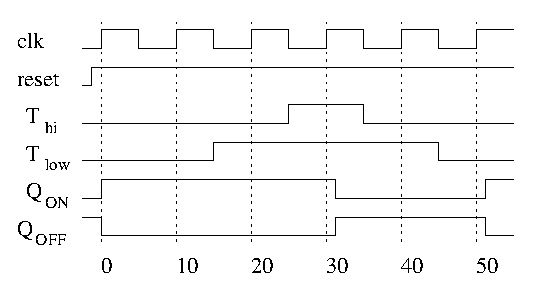
\includegraphics{./Fig7/FurnaceTime}}
\caption{A timing diagram for the furnace controller.}
\label{fig:FurnaceTime}

\end{figure}

The furnace controller is an example of a FSM whose states capture
the operating modes of a system.  The next example, the vending
machine, is a FSM whose states capture the history of the applied
inputs.

%%----------------VENDING MACHINE------------

\section{Vending Machine}
Consider the design of a FSM controlling the operation of a
very basic vending machine.  This machine is not a very user-friendly design
as it does not give out change.

\paragraph{Word Statement}
Design a FSM which has two inputs $N, D$ representing a nickel and a dime,
respectively.  $N=1$ when a nickel has been deposited and $D=1$ 
when a dime has been deposited. $N$ and $D$ never simultaneously are  
equal to 1 because a nickel and a dime cannot be simultaneously 
inserted into the coin slot.  The FSM has one output; it equals 1 
when 35\textcent~or more has been deposited.  After dispensing a
soda, the FSM should start collecting money for another soda.

\paragraph{State Diagram}
Usually two natural choices can be phrased for what the 
FSM is to remember.
\begin{enumerate}
\item The number of nickels and dimes deposited.
\item The total amount of money deposited so far.
\end{enumerate}

Clearly, the second approach is going to yield a FSM with far fewer
states, fewer flip flops, and in all likelihood, less logic for the
MIEs.  Hence, use the second approach and move on to
defining the states.  The FSM has eight states:  
0\textcent, 5\textcent, $\ldots$ 35\textcent~each representing the total
amount of money deposited so far.  Clearly, 0\textcent~should be the 
reset state.  The complete FSM is shown in Figure~\ref{fig:vend}.

\begin{figure}[ht]

\center{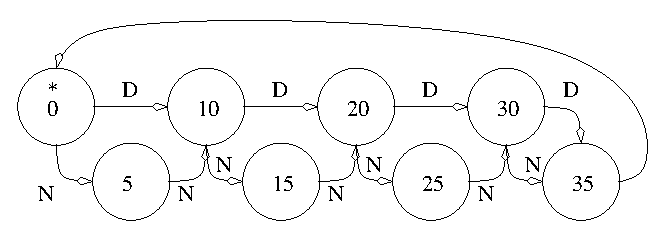
\includegraphics{./Fig7/VendSD}}
\caption{The state diagram for the vending machine.}
\label{fig:vend}

\end{figure}

The state diagram is not complete in the sense of the 
definition given on page~\pageref{page:completeness} because it does not
answer the question, ``What happen when no money is deposited?"
It should be obvious that from any state $S$, the transition
arcs labeled $N'$ or $D'$ point back to $S$.  In other words,
if no money is deposited, then the total amount of money
deposited does not change.  These arcs are omitted from the diagram for the
sake of clarity.  

Another interesting feature of the state diagram is the arc 
leaving state 35\textcent.  The arc is not labeled because 
this arc represents an unconditional state transition; the condition on
the arc is assumed to be true regardless of the input 
condition.  The FSM spends only one clock cycle in this
state, dispensing a single soda, before transitioning back to state
0\textcent.  

Finally, the FSM is not very user-friendly.  A user who deposits 
10\textcent~after depositing 30\textcent~gets a soda, but
no change.  The improvement of the FSM is left for a homework 
problem.  

\paragraph{Circuit Diagram}
The design process of a FSM consists of three steps, determining the 
number of flip flops, determining the MIEs, and determining the OEs.  
Since the FSM has eight states, the FSM will have eight flip flops, 
labeled 0\textcent, 5\textcent, $\ldots$ 35\textcent.  

In writing the MIEs, remember every state {\bf S} that has an outgoing 
arc labeled $N$, also has an undrawn arc labeled $N'$.  This undrawn 
arc leaves state {\bf S} and returns to state {\bf S}.  That is, if a nickel
is not deposited, then the FSM stays in the same state.  Likewise
every state which has an outgoing arc labeled $D$, has an undrawn self arc
labeled $D'$.  For example, three arcs terminate at state 5\textcent.
They are the arc from state 0\textcent labeled $N$ and the two arcs
leaving from state 5\textcent~labeled $N'$ and $D'$.  Hence the MIE
for state 5\textcent~is
$D_{5} = Q_{0}N + Q_{5}N' + Q_{5}D'$ which
can be simplified to 
$D_{5} = Q_{0}N + Q_{5}(N' + D')$.  The complete
list of MIEs is given below.


\begin{tabular}{l}

$D_{35} = Q_{25}D + Q_{30}N + Q_{30}D$ \\
$D_{30} = Q_{20}D + Q_{25}N + Q_{30}(N'+D')$ \\
$D_{25} = Q_{15}D + Q_{20}N + Q_{25}(N'+D')$ \\
$D_{20} = Q_{10}D + Q_{15}N + Q_{20}(N'+D')$ \\
$D_{15} = Q_{5}D +  Q_{10}N + Q_{15}(N'+D')$ \\
$D_{10} = Q_{0}D +  Q_{5}N  + Q_{10}(N'+D')$ \\
$D_{5}  =           Q_{0}N  + Q_{5}(N'+D')$ \\
$D_{0}  = Q{35} + Q_{0}(N'+D')$ \\

\end{tabular}

A table listing all the states and their output values could be built,
but an inspection of the word statement reveals that the FSM only
outputs 1 when 35\textcent~has been deposited.  Hence, the FSM should
output 1 when it is in state 35\textcent.  Consequently, $Z=Q_{35}$.

%%----------------Wait States------------

\section{Waits States}
When a FSM needs to interface with an entity operating much
slower than the FSM or with an event taking an unknown amount 
of time to happen, it is often necessary to include wait states in 
the FSM.  A wait state is exactly what its name implies, a state in
which the FSM waits for some input event to occur.

For example, imagine  constructing a FSM to control
a vending machine dispenser.  The FSM asserts its dispense output, 
enabling the vending machine to dispense a bag of chips, until its 
photodetector detects a bag of chips passing down the
dispense chute.  The photodetector input to the FSM is called
$photo$ and the dispense signal is an output from the FSM.

This FSM has a (wait) state with a self loop labeled 
$photo'$ in which it asserts the dispense output.  The FSM is
waiting for the $photo$ input to go to 1, signaling the bag of
chips is being dispensed.  While the \verb+photo+ signal is equal to 
0, the FSM asserts the dispense output.  The wait state should have
a second transition arc labeled \verb+photo+ which takes the FSM out
of the wait state when $photo$ equals 1.

The next section illustrates how to incorporate wait states into 
a FSM so that it waits patiently for cows to make their way through a 
cattle chute.

%%----------------DAISY------------
\section{DAISY}
Consider the design of a FSM capturing the current step of a 
process. The task is to design a high-tech cow-tracking system
for a local dairy. The system is called the Dairy Automated Information 
SYstem, or DAISY for short.  The system operates as follows.

\paragraph{Word Statement}
Cows have a RFID tag attached to their collars.  When the cow passes through the 
cattle chute on their way into the barn, a RFID reader reads the unique 
ID stored on the RFID tag and logs the cow into the barn.  The RFID 
system outputs a single bit: a 1 means the system has read an 
RFID tag and has successfully checked a cow back into the barn; a 0 means 
the RFID system is either still processing a tag or is not 
currently reading a tag.

In order to ensure each cow is scanned, the flow of cows
into the barn is controlled by two gates at either end of the chute.  Each 
gate is controlled by a single bit. To lift a gate, this input must be 
held at logic 1; to lower a gate, the input must be held at a logic 0.
The sequence of raising and lowering the gates in order to control the 
flow of cows is illustrated in Figure~\ref{fig:daisy}.

\begin{figure}[ht]
\center{\scalebox{0.5}{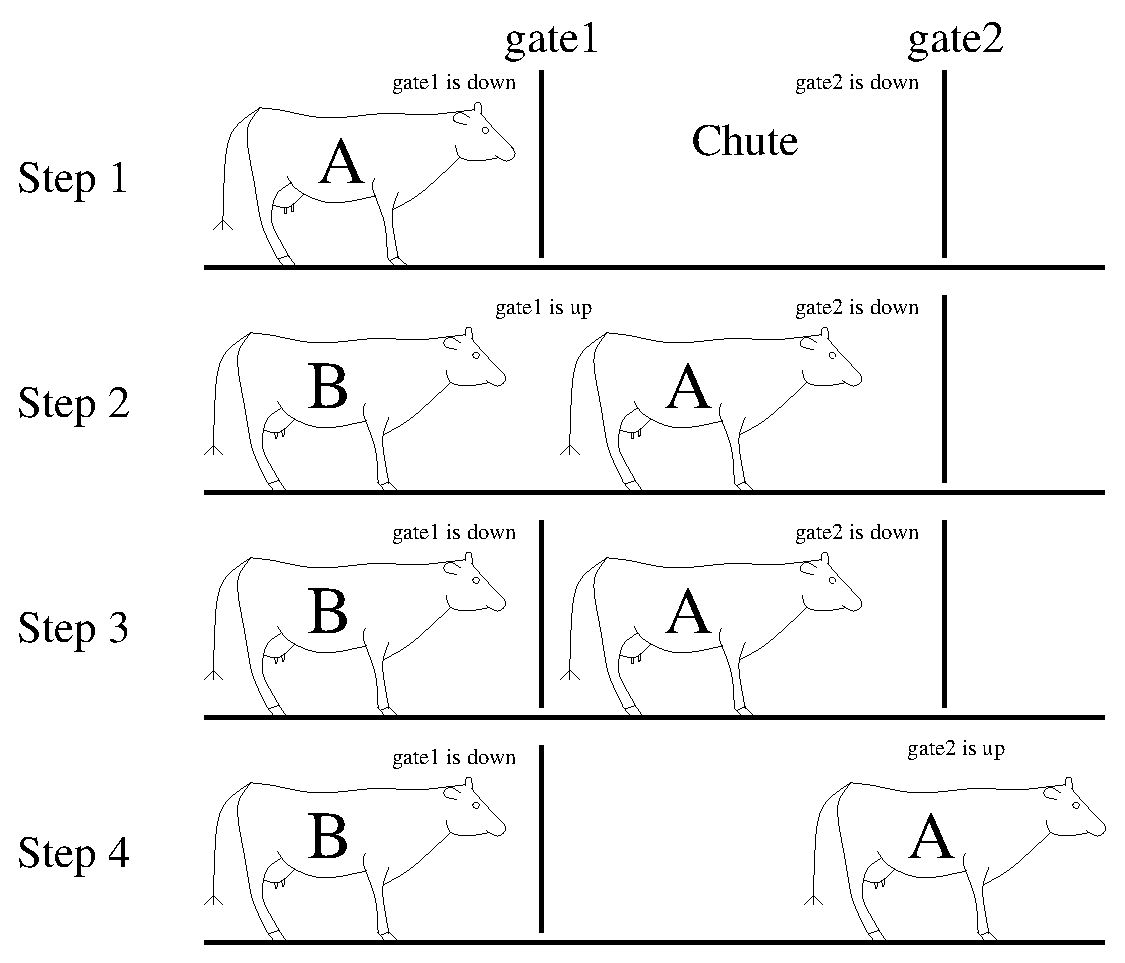
\includegraphics{./Fig7/Daisy}}}
\caption{The sequence of steps to gate a cow through the RFID reader chute.}
\label{fig:daisy}
\end{figure}

In Step 1, $gate1$ is lifted allowing cow $A$ to enter the chute.
In Step 2, the DAISY system has detected cow $A$ is in the chute and 
closes $gate1$.  The cow waits in the closed off chute until the RFID 
reader signals that it has read the tag and checked in cow $A$.  The DAISY system
then raises $gate2$ and waits for cow $A$ to leave the chute before closing $gate2$ 
and transitioning back to Step 1.  If the cow takes more than 30 seconds 
to leave the chute, then the cow is ``goosed" by a three-second burst of compressed air.
The compressed air is released by an electronically-controlled valve; 
asserting a 1 on the valve's input holds the value open, asserting a
0 closes the air valve.
The system then waits another 30 seconds before firing the air
valve again.  This process continues until the cow leaves the chute.
At any time when the cow leaves the chute, the cycle is 
interrupted and the DAISY system transitions back to Step 1.

In order to give DAISY an accurate sense of time, the system is
provided with a single timer with two bits of input and one bit of
output.  To use this timer, set the timer to either 3 or
30 seconds.  By asserting a set command for a single
clock cycle, the timer is set.  Then, the control input commanding the timer to count
down is continuously applied.  The output of the timer will equal
0 until the set time limit has expired at which times its output
will stay at 1 until a new time interval is set. 

Before deriving the state diagram, the inputs and outputs of
the DAISY system are categorized.

\paragraph{System Inputs and Outputs}
The word statement infers the existence of three inputs.  The RFID 
scanner sends the DAISY system a single bit which indicates if the cow has been
processed.  A second input tells the DAISY system if a cow is in
the chute. The final system input comes from a timer used
to inform the DAISY system when 3 or 30 seconds have expired.
\\ \\
\begin{tabular}{c|c|c}
RFID Scanner = $r$	& Cow Present = $c$	& Timer Status = $t$	\\ \hline \hline
1 - Cow checked in	& 1 - cow present	& 1 - timer up		\\ \hline
0 - Cow not processed	& 0 - no cow		& 0 - timer running	\\ 
\end{tabular}
\\ \\
The word statement infers the existence of four, separate outputs.  The gates in the
DAISY system are controlled by a single bit each.  Assume
a logic 1 must be continuously applied to a gate in order to keep it raised. In order
to use the timer, set it to either 3 or 30 seconds by applying 01 or
10 for a single clock cycle.  Then, the timer is run by applying 11.  The timer
outputs a status signal (a DAISY input) which should be monitored to tell
DAISY when the set time limit has expired.  When the electronic valve
controlling the compressed air is open, air rushes out, goosing the cow.
\\ \\
\begin{tabular}{c|c|c|c}
Gate1		& Gate2		& Timer Control			& Air Valve	\\ \hline \hline
1 - gate up 	& 1 - gate up	& 00 Stop timer			& 0 closed	\\ \hline
0 - gate down	& 0 - gate down	& 01 Set timer to 30 seconds	& 1 open	\\ \hline
		&		& 10 Set timer to 3 seconds	&		\\ \hline
		&		& 11 Run timer			&		\\
\end{tabular}

\paragraph{State Diagram}
The process of creating the state diagram for the DAISY system 
requires considering movement through the steps of the process required
to get a single cow through the gated chute.  Each step in this 
process then becomes a state or a set of states.  Each state 
asserts some output to control the devices connected to 
the DAISY system.  Below is one possible list; other arrangements are possible.

\begin{enumerate}
\item Open gate1
\item Wait for cow to enter chute
\item Close gate1
\item Wait for RFID to read cow
\item Open gate2
\item Wait for cow to leave
\item If 30 seconds has transpired, then ``goose" cow; goto Step 6 
\item Else if the cow has left, then close gate2; goto Step 1
\end{enumerate}

In order to simplify the labels on the state diagram arcs, the inputs 
are abbreviated. The RFID scanner input is represented by the variable $r$,
the cow present input is represented by the variable $c$, and the timer 
status input is represented by the variable $t$.

\begin{figure}[ht]

\center{\scalebox{0.7}{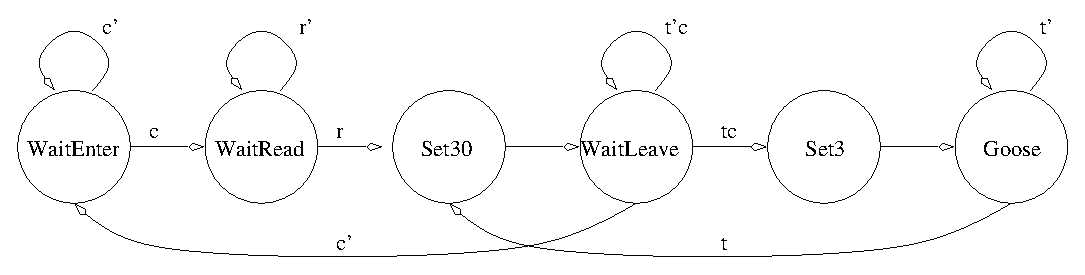
\includegraphics{./Fig7/DaisySD}}}
\caption{The state diagram for the DAISY system.}
\label{fig:daisySD}

\end{figure}

In some cases the FSM combines a couple of the items
in the list together into a single state.  For example,
Item 1 and Item 2 on the list, ``open gate1" and ``wait for cow 
to enter chute" are performed in the {\bf WaitEnter} state.  The
``Open gate1" action is performed by asserting the $gate1$
output while in this state.  The ``Wait for cow" action is
performed by the self arc labeled $c'$.  That is, while $c'$ is
true (while $c=0$), the FSM waits in the {\bf WaitEnter} state.
After a cow moves into the chute, the system moves into state
{\bf WaitRead}.  This state handles Item 3 and Item 4 in the list, 
``Close gate1" and ``Wait for RFID to read cow".  Closing the gate
is handled by asserting 0 on the $gate1$ output, while
waiting for the RFID reader is handled by the self arc labeled
$r'$.  When the RFID reader has checked in the cow, the 
FSM transitions to the state {\bf  Set30} where a 30-second count-down is
set.  The FSM then waits for the timer to time-out or for
the cow to leave.

The combinations of timer status and cow present while in the 
state {\bf WaitLeave} deserves some attention. The state has four 
combinations of these two inputs which effect the next state.  
In order to reason out the consequences of each input 
combination, structuring the analysis can be achieved by putting all 
four combinations of inputs into a truth 
table.  Then, each combination can be carefully analyzed to 
determine which next state occurs as well as to simplify the
expressions placed on the arcs.

\begin{table}
\begin{tabular}{c|c||c|c}
Timer Status 	& Cow Present 	& Action		& Next State	\\ \hline \hline
0			& 0			& close gate2	& WaitEnter		\\ \hline
0			& 1			& wait		& WaitLeave		\\ \hline
1			& 0			& close gate2	& WaitEnter		\\ \hline
1			& 1			& goose the cow	& Set3, Goose		\\ 
\end{tabular}
\end{table}

The pair of transitions which lead to the {\bf WaitEnter} state can be
simplified by noting that in both cases, the cow present status
bit is 0 (denoted by $c'$ on the state diagram).

\paragraph{Memory Input Equations}
Since the FSM is built with a one-hot encoding of the states, 
then the MIEs are formed by answering the question, ``How did 
I get into this state?"  The answer to this question, answered 
for each state is given below.

\begin{tabular}{l}
$D_{WaitEnter}	= Q_{WaitEnter}c' + Q_{WaitLeave}c'$  \\
$D_{WaitRead}	= Q_{WaitEnter}c + Q_{WaitRead}r'$ \\
$D_{Set30}	= Q_{WaitRead}r + Q_{Goose}t$ \\
$D_{WaitLeave}	= Q_{Set30} + Q_{WaitLeave}t'c$ \\
$D_{Set3}	= Q_{WaitLeave}tc$ \\
$D_{Goose}	= Q_{Set3} +  Q_{Goose}t'$ \\
\end{tabular}

\paragraph{Output Equations}
The output table is shown in Table~\ref{table:daisy}.  The table is
referred to as the {\it control word} table.  The term 
``control" is used because the table describes how the FSM controls 
its associated hardware.  The term ``word" is used to indicate 
the control is formed from a collection of bits.

\begin{table}[ht]
{\small
\begin{tabular}{c||c|c|c|c}
State		& Gate1		& Gate2		& Timer Control			& Air		\\ \hline \hline
		& 1 - gate up	& 1 - gate up	& 00 Stop timer			& 0 - closed \\ \hline
		& 0 - gate down	& 0 - gate down	& 01 Set timer to 30 seconds	& 1 - open	\\ \hline
		&			&			& 10 Set timer to 3 seconds	&		\\ \hline
		&			&			& 11 Run timer			& 		\\ \hline \hline
{\bf WaitEnter}	& 1			& 0			& 00					& 0		\\ \hline
{\bf WaitRead}	& 0			& 0			& 00					& 0		\\ \hline
{\bf Set30}		& 0			& 0			& 01					& 0		\\ \hline
{\bf WaitLeave}	& 0			& 1			& 00					& 0		\\ \hline
{\bf Set3}		& 0			& 0			& 10					& 0		\\ \hline
{\bf Goose}		& 0			& 0			& 11					& 1		\\
\end{tabular}
}
\label{table:daisy}
\end{table}

The output equations are derived by looking at the columns
of the control word table.  Each column is given its own
output equation by asking, ``What states cause this 
output to go to 1?"  ORing together these states produced
the output equation for the corresponding output.  For 
example, the $Gate1$ output only goes to logic 1 when the 
FSM is in the {\bf WaitEnter} state, hence 
$Z_{Gate1} = Q_{WaitEnter}$.  The complete list of output 
equations is given below.

\begin{tabular}{l}

$Z_{Gate1}	= Q_{WaitEnter}$  \\
$Z_{Gate2}	= Q_{WaitLeave}$ \\
$Z_{Timer1}	= Q_{Set3} + Q_{Goose}$ \\
$Z_{Timer0}	= Q_{Set30} + Q_{Goose}$ \\
$Z_{Air}	= Q_{Goose}$ \\
\end{tabular}

\section{Exercises}
\section{Exercises}
\label{section:finiteStateMachines}
\graphicspath{ {./chapter07/FigHw} }

\begin{enumerate}
\item A finite state machine has been implemented with four
flip-flops, two inputs and three outputs. 
	\begin{enumerate}
	\item What are the minimum and maximum number of states in the diagram?
\begin{onlysolution}  \textbf{Solution} \itshape{
Since there are three flip flops we can have a maximum of 8 states.  The minimum
number of states is a bit tricky.  A practical answer is 5, because if you
had fewer states you would use fewer flip flops.  However, the question
asks for a minimum, in which case you could have 1 state.  Note, that a
1 state FSM would only generate a single output and hence would not be a
very interesting circuit.
}\end{onlysolution} 
	\item What are the minimum and maximum number of transition arrows 
		starting at a particular state?
\begin{onlysolution}  \textbf{Solution} \itshape{
These values are the same.  Since there are two bits of input there are four
different inputs that can be applied at each state.  Thus, four arrows must
leave each state.
}\end{onlysolution} 
	\item What are the minimum and maximum number of transition arrows 
		ending in a particular state?
\begin{onlysolution}  \textbf{Solution} \itshape{
In a typical design your systems will have a reset state, it normal for such
states to have NO input arcs.  You only visit them when the power is turned on.
This is the minimum number of arcs that can terminate at a state.  On the
other hand, I could image a machine where   transition arc points to a
particular state (not a very interesting FSM).  Hence all 32 arcs could point
to a single state.
}\end{onlysolution} 
	\item What are the minimum and maximum number of different binary patterns
		that are displayed on the outputs? 
\begin{onlysolution}  \textbf{Solution} \itshape{
this is a tricky question, you need to determine which of the inputs and outputs
constrains the number of distinct patterns on the output.  You should consult
figure 7.1 for some guidance.  There are three bits of output which have the possibility
of generating 8 different outputs.  There are a total of six bits of input to the
combinational logic box, more than enough to cope with the 8 different output.  On
the other end of the scale, I can imagine a FSM which only produces a single output,
it would however, not be very interesting.
}\end{onlysolution} 
	\end{enumerate}


\item \textbf{ (20 points)}
The state assignment for a FSM influences the amount of
combinational logic required in the realization.  In the following
problem this phenomena is investigated.  Determine the MIEs 
for the following state table using
both the state assignments.

\begin{tabular}{lll}
State Table & State Assignment 1 & State Assignment 2  \\
\begin{tabular}{c|c|c}
CS x & 0    & 1    \\ \hline
A    & A,0  & B,0  \\ \hline
B    & C,1  & F,1  \\ \hline
C    & D,0  & C,0  \\ \hline
D    & A,1  & H,1  \\ \hline
E    & F,1  & E,1  \\ \hline
F    & G,0  & F,0  \\ \hline
G    & G,1  & C,1  \\ \hline
H    & D,1  & E,1  \\ 
\end{tabular}
& 
\begin{tabular}{c||c|c|c}
State & $Q_2$ & $Q_1$ & $Q_0$ \\ \hline
A     & 0     & 0     & 0     \\ \hline
B     & 0     & 0     & 1     \\ \hline
C     & 0     & 1     & 1     \\ \hline
D     & 0     & 1     & 0     \\ \hline
E     & 1     & 0     & 0     \\ \hline
F     & 1     & 0     & 1     \\ \hline
G     & 1     & 1     & 1     \\ \hline
H     & 1     & 1     & 0     \\ 
\end{tabular}
&
\begin{tabular}{c||c|c|c}
State & $Q_2$ & $Q_1$ & $Q_0$ \\ \hline
A     & 0     & 0     & 0     \\ \hline
B     & 1     & 1     & 1     \\ \hline
C     & 0     & 0     & 1     \\ \hline
D     & 1     & 1     & 0     \\ \hline
E     & 1     & 0     & 1     \\ \hline
F     & 0     & 1     & 1     \\ \hline
G     & 1     & 0     & 0     \\ \hline
H     & 0     & 1     & 0     \\ 
\end{tabular}
\end{tabular}

After obtaining the MIEs for both realizations, determine the cost 
of each solution according to the following formula: 
$C(FSM) = A + O + 6*F$.  Where $C(FSM)$ denotes
the cost of the FSM, 
$A$ is the cost of the AND gates,  
$O$ is the cost of the OR gates, and 
$F$ is the number of flip flops.  
The cost of an AND gate is equal to the number of inputs to the 
AND gate.  Likewise the cost of an OR gate is equal to the number
of inputs.  NOT gates are free. For example, the circuit 
$A'B + ABC'$ costs $2+3+2=7$.  

Submit:
\begin{enumerate}
\item Shared steps of the design process.
\item Derive the MIEs for each of the two realizations.
\begin{onlysolution}  \textbf{Solution} \itshape{

State Assignment 1

\begin{tabular}{l|l|l|l|l}
$Q_2 Q_1 \ Q_0 x$  & 00 & 01  & 11 & 10 \\ \hline
00  & 000,0 & 001,0 & 101,1 & 011,1  \\ \hline
01  & 000,1 & 110,1 & 011,0 & 010,0  \\ \hline
11  & 010,1 & 100,1 & 011,0 & 111,1  \\ \hline
10  & 101,1 & 100,1 & 101,0 & 111,0  \\ 
\end{tabular}

$D_2 = Q_1Q_0'X + Q_1'Q_0X + Q_2Q_0X' + Q_2Q_1'$		\\
$D_1 = Q_2Q_1X' + Q_2'Q_1X + Q_1Q_0 + Q_0X'$			\\ 
$D_0 = Q_2Q_1'X' + Q_2'Q_1'X + Q_1'Q_0 + Q_2Q_0 + Q_0X$ 	\\    
$Z   = Q_2'Q_1'Q_0 + Q_1Q_0' + Q_2Q_0' + Q_2Q_1$		\\ 

State Assignment 2

\begin{tabular}{l|l|l|l|l}
$Q_2 Q_1 \ Q_0 x$  & 00 & 01  & 11 & 10 \\ \hline
00  & 000,0 & 111,0 & 001,0 & 110,0  \\ \hline
01  & 110,1 & 101,1 & 011,0 & 100,0  \\ \hline
11  & 000,1 & 010,1 & 011,1 & 001,1  \\ \hline
10  & 100,1 & 001,1 & 101,1 & 011,1  \\ 
\end{tabular} 

$D_2 = Q_2Q_1'Q_0'X' + Q_2Q_1'Q_0X + Q_2'Q_1Q_0' + Q_2'Q_0'X + Q_2'Q_0X'$ \\
$D_1 = Q_2'Q_1Q_0'X' + Q_2'Q_1'Q_0'X + Q_2Q_1X+Q_1Q_0X + Q_1'Q_0X'$\\
$D_0 = Q_1'X + Q_2'X + Q_2Q_0$					\\
$Z   = Q_1Q_0' + Q_2$						\\

}\end{onlysolution} 


\item Determine the cost of each of the two realizations.

\begin{onlysolution}  \textbf{Solution} \itshape{
\begin{tabular}{l|l|l}
	& State Assignment 1	& State Assignment 2 \\ \hline
$D_2$	& 	15		&	22	\\ \hline
$D_1$	&	14		&	22	\\ \hline
$D_0$	&	17		&	9	\\ \hline
$Z$	&	13		&	4	\\ \hline
Total	& 6*3 + 59 = 77 		& 6*3 + 57 = 75	\\ 
\end{tabular}
}\end{onlysolution} 
\item Determine the cost of each of the two realizations using Espresso.
\begin{onlysolution}  \textbf{Solution} \itshape{
Espresso cost 77 for state assignment  1 \\
Espresso cost 75 for state assignment  2
}\end{onlysolution} 
\end{enumerate}

\item \textbf{ (8 pts.)} Realize the FSM in the previous problem using 
a one-hot encoding.  Determine
the MIEs and the cost of the circuit using the same metric.
It is helpful to convert the state table into a state diagram.
\begin{onlysolution}  \textbf{Solution} \itshape{
\begin{description}
\item $D_A = Q_AX' + Q_DX'$
\item $D_B = Q_AX$
\item $D_C = Q_BX'+Q_CX+Q_GX$
\item $D_D = Q_CX'+Q_HX'$
\item $D_E = Q_EX+Q_HX$
\item $D_F = Q_BX+Q_EX'+Q_FX$
\item $D_G = Q_FX'+Q_GX'$
\item $D_H = Q_DX$
\item $Z   = Q_B + Q_D + Q_E + Q_G + Q_H$
\end{description}

The cost of this solution is 6*8 + 6 + 2 + 9 + 6 + 6 + 9 + 6 + 2 + 5 = 48 + 51 = 99
}\end{onlysolution} 

\item \textbf{ (8 points)}
Enhance the vending machine discussed in this chapter as follows.
Add two buttons for a beverage selection; \textit{ regular} soda and \textit{ diet}
soda, see Figure~\ref{fig:Vend}.  This machine will have a change dispenser.  
If the user deposits more than 35\textcent, the circuit should send a signal to
either the \textit{ nickel change} dispenser or the \textit{ dime change} dispenser, 
a single bit sent for one clock cycle to a dispenser will yield a single coin.
When the user deposits 35\textcent (or more) the machine gives any change and 
then waits for one of the two buttons to be depressed.  Depending on the 
selection, the circuit should send a signal to either the 
\textit{ regular dispenser} or
the \textit{ diet dispenser} mechanism.  The dispenser need only get a signal for
one clock cycle.  After the dispensing, go back to the reset state.
\begin{figure}[ht]
\center{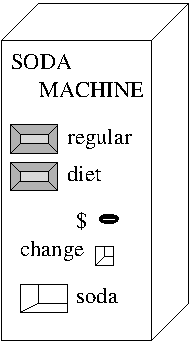
\includegraphics{Prob7-10}}
\caption{A basic vending machine.}
\label{fig:Vend}
\end{figure}

\begin{onlysolution}  \textbf{Solution} \itshape{

\begin{figure}[ht]
\center{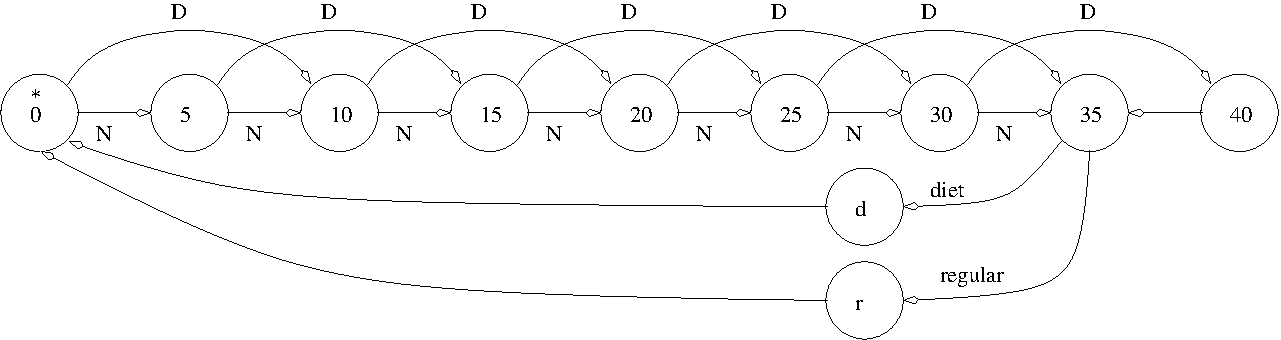
\includegraphics{Sol7-9}}
\end{figure}

Note, that in the figure if a input does not appear on
any arc emanating from a state then it is implied that
this input will have no effect on the next state.  Below
are the outputs for each of the states above.

\begin{tabular}{|l||l|l|l|} \hline
\multicolumn{4}{|c|}{outputs from the vending FSM}              \\ \hline \hline
state & nickel change	& diet dispense & regular dispense      \\ \hline
      & 0 give none	& 0 give none	& 0 given none		\\ \hline
      & 1 give nickel	& 1 dispense diet & 1 dispense regular	\\ \hline
      & 		&		&			\\ \hline
0     & 0		& 0		& 0			\\ \hline
5     & 0		& 0		& 0			\\ \hline
10    & 0		& 0		& 0			\\ \hline
15    & 0		& 0		& 0			\\ \hline
20    & 0		& 0		& 0			\\ \hline
25    & 0		& 0		& 0			\\ \hline
30    & 0		& 0		& 0			\\ \hline
35    & 0		& 0		& 0			\\ \hline
40    & 1		& 0		& 0			\\ \hline
d     & 0		& 1		& 0			\\ \hline
r     & 0		& 0		& 1			\\ \hline
\end{tabular}
}\end{onlysolution} 



\item \textbf{ (6 pts.)}
Build a FSM for a car alarm.  The input to the FSM
comes from a tilt sensor.  The tilt-sensor outputs 1 when the 
car has been physically displaced by a preset amount, otherwise the
tilt sensor outputs 0.  The output of the circuit drives an alarm,
when the alarm output equals 1 the alarm sounds, otherwise the alarm
does not sound.  Once the alarm has been set off, it will continue
sounding until a reset input equals 1, at which point the alarm will
stop sounding.

Draw the state diagram and from this determine the MIEs and OEs.


\item \textbf{ (12 pts.)}
Build a FSM which displays the revolutions per second
(RPS) of a motor.  The output shaft of the motor is attached to 
a sensor whose output pulses to logic 1 every time the motor's shaft
completes a single revolution.  This sensor signal is attached to
a counter.  The behavior of the counter to the pulse input is determined
by a 1-bit control input (coming from the FSM) given by the following 
truth table.

\begin{tabular}{l|l}
control & behavior \\ \hline \hline
0	& reset to 0 \\ \hline
1	& count up \\
\end{tabular}

The counter's output is eight bits wide, representing two BCD digits.  Thus,
the counter's output will go from 19 to 20 when the control input is 1
and there is a pulse on the sensor line.  This 8-bit output from the
counter is sent to the data input of an 8-bit register.  The register's
control input comes from the FSM.  The output of the register is split
into two nybbles (a 4-bit value is called a nybble)
each sent its own BCD to 7-segment converter.  In order to determine
when a second is up, the FSM is fed a reference signal denoted by 
the variable $R$ with a period of exactly 1Hz and a 50\% duty cycle; 
the duty cycle of a square wave is the proportion of time the signal 
spends at logic 1.   That is $R$ is at logic 1 for half a second and 
then at logic 0 for half a second.  The FSM is being supplied with a 
clock signal, $clk$, with a frequency much greater than 1Hz (perhaps 
in the MHz range).  The architecture of the FSM is given in 
the figure below.  

%% 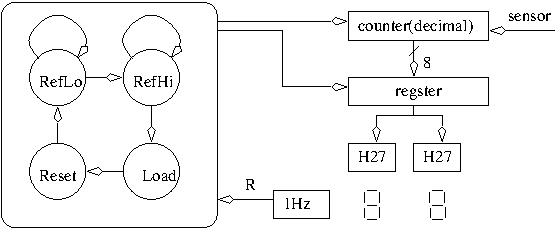
\includegraphics{RPS}

Submit:
\begin{enumerate}
\item Label the arcs of the FSM with R or R' so that the
 circuit operates correctly.
\item Determine the output for each state.  Instead of writing the
output in each state, list the outputs in the following control
word table.

\begin{tabular}{l||l|l}
state	& counter	& register \\ \hline 
	& 0 reset	& 0 hold \\ \hline
	& 1 count up& 1 reset \\ \hline \hline
RefLo	&		&	  \\ \hline
RefHi	&		&	  \\ \hline
Load 	&		&	  \\ \hline
Reset	&		&	  \\ 
\end{tabular}

\item Determine the output equations.
\item Determine the memory input equations assuming a one-hot
encoding of the states.
\end{enumerate}


\item \textbf{ (12 pts.)}
Build a digital circuit which controls an automatic garage door opener.  
The garage door circuit has three bits of input.  The first input, called 
$button$, comes from a the main control button used to open or close the 
garage door.  When pressed $button=1$ otherwise $button=0$.  The garage 
door rides in a track, at the top and bottom of of which are two 
limit switches.  The top limit switch equals 1 when the garage door 
is all the way up, otherwise its output equals 0.  The bottom limit 
switch equals 1 when the garage door is all the way down, otherwise 
its output equals 0.  The garage door circuit has two bits of output 
called $motor$.  When $motor=01$, the motor moves the door in a downward 
motion, closing the door.  When $motor=10$, the motor moves the door 
upward, opening the garage door.  When $motor=00$, the motor is turned off.

\begin{figure}[ht]
%% \center{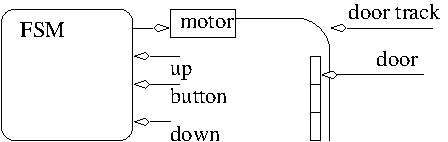
\includegraphics{./FigWork/Door}}
\caption{The garage door and the circuit controlling it.}
\label{fig:hwgarage}
\end{figure}

Construct the FSM assuming a one-hot encoding of the states.
Determine the memory input equations and output equations.


\begin{onlysolution}  \textbf{Solution} \itshape{

\paragraph{Control unit}
The control unit includes so called wait states.  Waits states are
a result of the fact that the clock running the FSM is usually 
much faster than the physical phenomena being monitored by the FSM.
Unless told otherwise, you can assume that any FSM that you are 
building has a clock which operates on the order of megahertzs.
This means that the resulting FSM can make around 1 million 
state transitions per second.  Clearly, a garage door needs more
than one millionth of a second to open or close.  Consequently, 
the FSM in this problem needs to wait for the door to be opened.
This is done by having the FSM repetitively check the status of the
door via the up or down limit switches.  In addition to waiting 
for the garage door to open and close the FSM must wait for a 
button press.

\begin{figure}[ht]
%\center{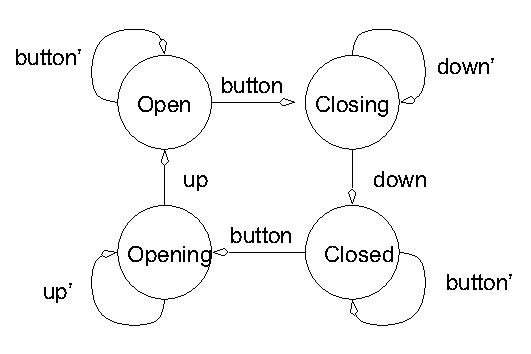
\includegraphics{../Fig/GarageFSM}}
\caption{The FSM for the garage door controller.}
\end{figure}

The state diagram for the garage door controller has four states.
In the open and close state, the FSM is waiting for a button push,
while the button is not pressed the door stays open or closed.  As
soon as the button is pressed the door starts to open or close.
It stays in this state until the limit switches tell the FSM that
the door has reached the limit of its travel.

\paragraph{Memory Input Equations}
Since we are building the garage door controller assuming a
one hot encoding of the states, each state will get its own
flip flop.  Each flip flop will output a 1 when the FSM is 
in that state.  The memory input equations for a particular
state are determined by answering, ``how do you get into that 
state?" The four answers to this questions are provided below.

\begin{tabular}{l}
$D_{open} = Q_{open}button' + Q_{opening}up$ \\
$D_{close} = Q_{close}button' + Q_{closing}down$ \\
$D_{opening} = Q_{close}button+ Q_{opening}up'$ \\
$D_{closing}  = Q_{open}button+ Q_{closing}down'$ \\
\end{tabular}


\paragraph{Output Equations}
The outputs for complex FSMs are usually not written inside the
states, rather a separate table is constructed which contains the
output for each state.   Even though this is a simple example
we will construct an output table.

\begin{tabular}{l|l}
State	& motor		\\ \hline
	& 00 stop	\\ \hline
	& 01 down	\\ \hline
	& 10 up		\\ \hline
open    & 00 		\\ \hline
close   & 00		\\ \hline
opening & 10 		\\ \hline
closing & 01 		\\ 
\end{tabular}

Call the outputs $Z_{m1}$ and $Z_{m0}$, for the most and least
significant bits of the output respectively.  Then the outputs
are determined by asking for which states does the output
equal 1?  The answers to this question are shown below.

\begin{tabular}{l}
$Z_{m1} = Q_{opening}$ \\
$Z_{m0} = Q_{closing}$ \\
\end{tabular}

}\end{onlysolution} 


\item \textbf{ (8 pts.)}
Build a digital circuit to control a single traffic light.  The circuit
has three outputs, $Rlight, Ylight$ and $ Glight$.  When
$Rlight=1$ the red light illuminates otherwise the light is off.
The same behavior holds true for $Ylight$ and $Glight$.  In order
to sequence the lights, the circuit has three timers, Rtimer, Gtimer and 
Ytimer.  Each timer controls the length of time that its light should be 
illuminated.  Each timer has one bit of input and one bit of output.  When a 
timer's input is 0, the timer is reset.  When a timer's one bit
input is 1, the timer 
counts down its preset timer interval.  When a timer counts all the way down,
its output goes to 1 and stays there until the timer is reset (by applying
an input of 0).  The state diagram of the circuit is shown in the
figure below.  As shown in this figure the FSM receives input from the 
three timers, while the output of the FSM controls the counters. Complete
the following three tasks.

% 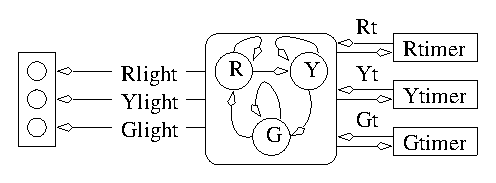
\includegraphics{./FigWork/Light}

\begin{enumerate}
\item Label the arcs of the FSM with the input values (Rt, Yt or Gt)
needed to make the circuit operate correctly.  

\item Next, determine what the output should be in each
of the states.  Instead of writing the output in each state, the
outputs are organized in a separate table.  In this table, each
row will contain the output associated with a particular state.
Each column in the table will be associated with one bit of the output.

\begin{tabular}{l||l|l|l|l|l|l}
state	& Rlight & Ylight & Glight & Rtimer & Ytimer & Gtimer	\\ \hline 
	& 0 off  & 0 off  & 0 off  & 0 rst  & 0 rst  & 0 rst	\\ \hline
	& 1 on   & 1 on   & 1 on   & 1 run  & 1 run  & 1 run	\\ \hline \hline
R	&	 &	  &	   &	    &	     &		\\ \hline
Y	&	 &	  &	   &	    &	     &		\\ \hline
G	&	 &	  &	   &	    &	     &		\\ 
\end{tabular}

\item Finally, write the memory input equations and output 
equations for the traffic light controller.  In order to write the
memory input equations use the labels on the state transitions from 
the state diagram.   In order to write the output equations 
use the output table.

\begin{tabular}{p{2in}p{2in}}
        \begin{tabular}{l}
        $Q_{red}$= \\
        $Q_{yellow}$= \\
        $Q_{greew}$= \\
        \end{tabular} 
&
        \begin{tabular}{l}
        $Z_{Rlight}$= \\
        $Z_{Ylight}$= \\
        $Z_{Glight}$= \\
        $Z_{Rtimer}$= \\
        $Z_{Ytimer}$= \\
        $Z_{Gtimer}$= \\
        \end{tabular}
\end{tabular}
\end{enumerate}

\item \textbf{ (16 pts.)}
Build a FSM which make the hexapod robot shown in Figure~\ref{fig:hexapod}
walk forward.

\begin{figure}[ht]
\center{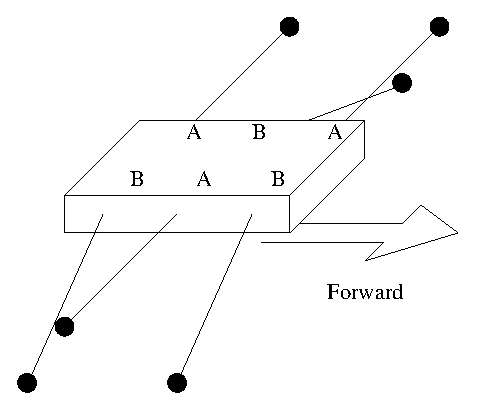
\includegraphics{Prob7-11}}
\caption{A hexapod walking robot.}
\label{fig:hexapod}
\end{figure}

Each leg of the hexapod robot is moved by two nitinol (Flexinol) wires.  
At rest, nitinol wire is straight.  When 5 volts (logic 1) is applied to 
the wire, it bends in a particular direction.  The two wires making up
a particular leg are positioned so that they move in perpendicular
directions.  One wire moves a leg up or down and the other will move 
the wire forward or backwards.  The table below elaborates.

\begin{tabular}{l|l|l}
wire   & logic 0 & logic 1	\\ \hline
$w_0$  & down	 & up		\\ \hline
$w_1$  & forward & backward	\\ 
\end{tabular}

The hexapod robot walks by moving three legs in unison; see $A$ and
$B$ in Figure~\ref{fig:hexapod}.  The movements of $A$ and $B$ are
coordinated so that, at times, the hexapod is balanced on three legs.
A portion of the walking gait is shown in Figure~\ref{fig:hexgate};
note that in this figure the viewer is looking down at the top of the 
robot which is moving to the right.  The dotted legs are assumed to be in
the air, solid legs are in contact with the ground.

\begin{figure}[ht]
\center{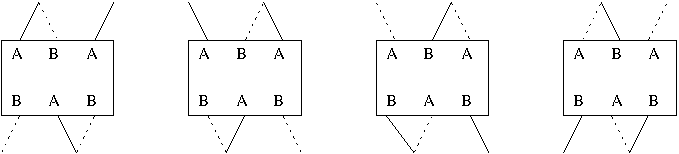
\includegraphics{Prob7-11b}}
\caption{The walking gait of the hexapod robot.}
\label{fig:hexgate}
\end{figure}

Assume that the legs can move to their correct position in one clock
cycle.  Define each state as a position of the legs in 
Figure~\ref{fig:hexgate}. Draw the state diagram,
and determine the memory input and output equations.

\begin{onlysolution}  \textbf{Solution} \itshape{

\begin{figure}[ht]
\center{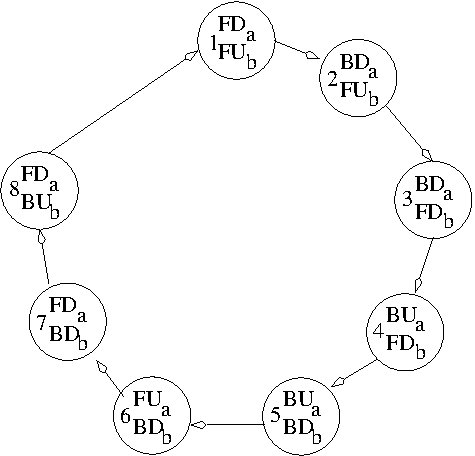
\includegraphics{Sol7-11}}
\end{figure}

Note that the states have been given numbers to simplify the
description of the states.  Here is a listing of the outputs 
associated with each state:

\begin{tabular}{l|l|l|l|l}
State  & $Aw_1$ & $Aw_0$ & $Bw_1$ & $Bw_0$  \\ \hline
1	& 0	& 0	 & 1	  & 1		\\ \hline
2	& 1	& 0	 & 0	  & 1		\\ \hline
3	& 1	& 1	 & 0	  & 0		\\ \hline
4	& 0	& 1	 & 1	  & 0		\\ 
\end{tabular}

\textbf{ MIEs and OEs}

\begin{tabular}{ll}
MIEs		&	OEs			\\
$D_1 = D_4$	&	$Z_{Aw_1} = Q_2 + Q_3$	\\
$D_2 = D_1$	&	$Z_{Aw_0} = Q_3 + Q_4$	\\
$D_3 = D_2$	&	$Z_{Bw_1} = Q_1 + Q_4$	\\
$D_4 = D_3$	&	$Z_{Bw_0} = Q_1 + Q_2$	\\
\end{tabular}

}\end{onlysolution} 

\item \textbf{ (12 pts.)}
\label{item:robot}
Build a FSM which makes the simple robot shown in Figure~\ref{fig:Robot}
move along (track) the black line crossing two intersections.
\begin{figure}[ht]
\center{\scalebox{0.8}{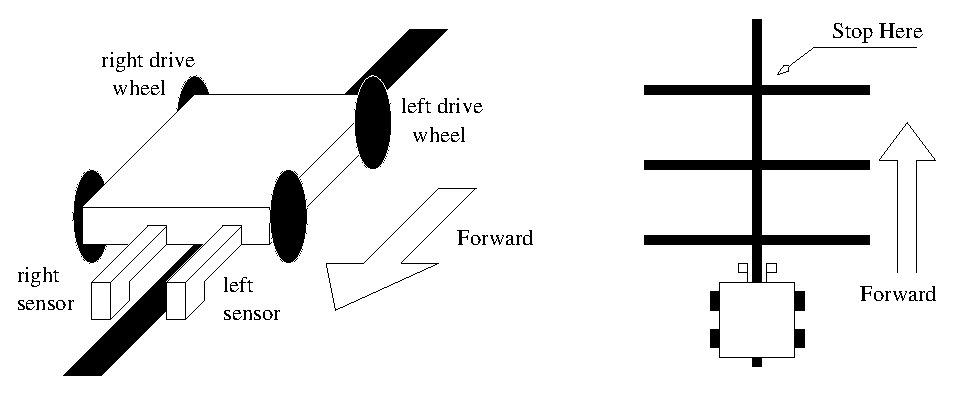
\includegraphics{Prob7-12}}}
\caption{A simple line-tracking robot that must cross two intersections.}
\label{fig:Robot}
\end{figure}

The FSM has two inputs, a left sensor, denoted \textit{ ls}, and a right 
sensor, denoted \textit{ rs}.  These two sensors look down at the ground.  
When a sensor sees white, it outputs 0; when it see black, it outputs 1.  
The sensors are spaced far enough apart that they can straddle the black 
line and see white on either side.  The FSM has two outputs, a left
motor, denoted \textit{ lm} and a right motor, denoted \textit{ rm}.  A motor
rotates when it is sent a 1 and does not rotate when it is sent a 0.
The FSM should constantly check that the robot is straddling the line.
If it is not the FSM should take corrective action by stopping one of
the wheels.

Submit the state diagram for the FSM,  MIEs and OEs using 
a one-hot encoding of the states.

\begin{onlysolution}  \textbf{Solution} \itshape{
\begin{figure}[ht]
\center{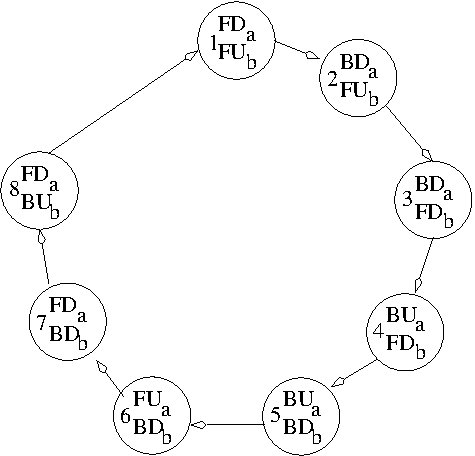
\includegraphics{Sol7-11}}
\end{figure}

\begin{tabular}{l|l|l|l}
State & lm		  & rm			\\ \hline
      & 0 stop left wheel & 0 stop right wheel  \\ \hline
      & 1 turn left wheel & 1 turn right wheel  \\ \hline
      &                   &                     \\ \hline \hline
Reset	 & 1		  & 1			\\ \hline
Straight & 1		  & 1			\\ \hline
Left     & 0		  & 1			\\ \hline
Right    & 1		  & 0			\\ \hline
OnLine   & 1		  & 1			\\ \hline
Up	 & 1		  & 1			\\ \hline
Stop	 & 0		  & 0			\\ 
\end{tabular}
} \end{onlysolution}  

\item \textbf{ (16 pts.)}
Make the robot from Problem \ref{item:robot} cross 63 intersections.
The problem is that the number of states will grow to large to handle
with a FSM by itself.  Additional hardware, in the form of a counter 
and comparator, are added to the FSM to address this problem.

\begin{figure}[ht]
\center{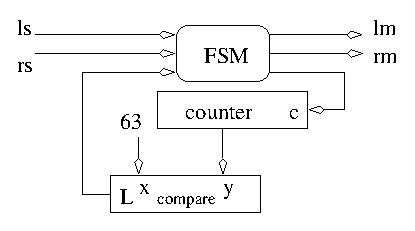
\includegraphics{Prob7-13}}
\caption{The innards of a intersection counting, line tracking robot.}
\label{fig:linecounter}
\end{figure}

Assume that the counter is reset to 0 when the circuit
is first turned on.  The robot must still track the line, but
must also count up once every time it crosses an intersection.  Remember
the digital circuit shown in Figure~\ref{fig:linecounter} is
operating much faster than the robot is crossing intersections.
The state diagram needs to have wait states while it crosses
the intersection, similar to those
in the DAISY example.  Assume the counter counts up
when the control input is 1 and the clock rises.  When the control
input is 0, then the counter holds its current count value.

Submit the state diagram for the FSM, OEs and MIEs for a one-hot 
encoding of the states.  

\begin{onlysolution}  \textbf{Solution} \itshape{
\pagebreak
If you encoded 64 line crossing using only a FSM you would have
on the order of 256 states, 4 for each line crossing.  The solution
is to use a counter to keep track of how many lines have been crossed.
The states below explain.

\textbf{ DP \& CU}

\begin{figure}[ht]
\center{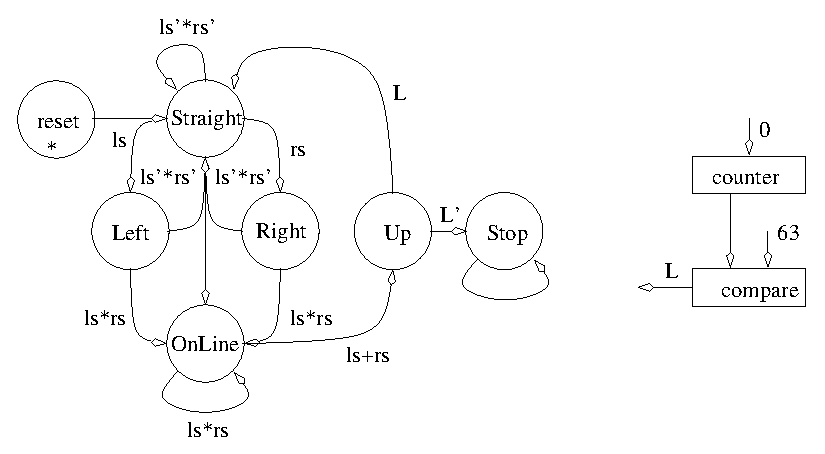
\includegraphics{Sol7-12}}
\end{figure}

\textbf{ Control Word}

\begin{tabular}{l|l|l|l}
State & lm		  & rm			& counter \\ \hline
      & 0 stop left wheel & 0 stop right wheel  & 00 hold \\ \hline
      & 1 turn left wheel & 1 turn right wheel  & 01 load \\ \hline
      &                   &                     & 10 count\\ \hline \hline
Reset	 & 1		  & 1			& 01	  \\ \hline
Straight & 1		  & 1			& 00	  \\ \hline
Left     & 0		  & 1			& 00	  \\ \hline
Right    & 1		  & 0			& 00	  \\ \hline
OnLine   & 1		  & 1			& 00	  \\ \hline
Up	 & 1		  & 1			& 10	  \\ \hline
Stop	 & 0		  & 0			& 00	  \\ 
\end{tabular}

One could easily derive the MIEs and OEs for the FSM.
} \end{onlysolution} 

\item \textbf{ (24 pts.)}
Construct a digital circuit to control the operation of a
simple washing machine, see Figure ~\ref{fig:Wash}.
\begin{figure}[ht]
\center{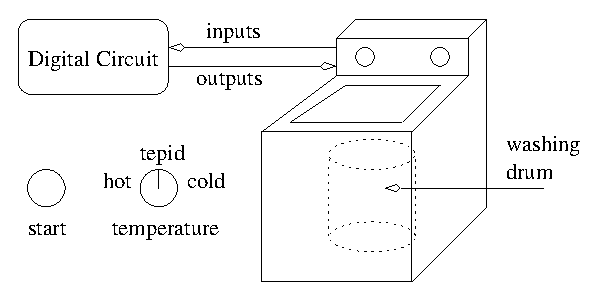
\includegraphics{Prob7-14}}
\caption{A humble washing machine with a close-up of the start
button and temperature switch.}
\label{fig:Wash}
\end{figure}
To use the simple washing machine set the temperature switch to 
either hot, tepid or cold and then press the start button.
To build a digital circuit to control the washing of clothes
its necessary to understand the washing cycle.  When the start
button is pressed water of the selected temperature pours 
into the washing drum.  The simple washing machine has two 
electronically controlled water valves, the hot valve admits 
hot water into the washing drum and the cold valve admits 
cold water.  Water continues to pour into the drum until it
fills.  There are two water level sensors; the full switch signals when 
the drum is full of water and the empty switch signals when the drum
is empty.  After the drum is full of water the simple washing machine
starts to agitate the clothes.  The simple washing machine has a motor 
controlled by two bits, which agitates (a rapid back and forth motion), 
spins (a rapid rotation in one direction) or does nothing.  After 
agitating for 15 minutes, the agitation cycle stops and
the machine drains its water.  Water leaves the drum through
a drain valve.  When the drum is emptied of water the washing machine enters
the rinse cycle.   The rinse cycle fills the drum with cold
water and agitates for 5 minutes.  The rinse cycle concludes
by draining the water from the drum.
When the drum is emptied of water the washing machine enters
the spin cycle.  This lasts for 5 minutes.  The simple washing machine 
keeps track of time  using a 5 minute timer.   To use the timer 
it must first be reset for one clock cycle.  After being reset the 
timer will count down as long as the timer input is set to run.  
After 5 minutes have elapsed the timer output will go to logic 1 and 
stay there until the timer is reset.  In order to get longer time
intervals, the timer should be reset for another 5 minutes and count 
down again.  When the spin cycle is done, the washing is complete. The 
inputs from the washing machine to the digital circuit have the 
following meaning.

\begin{tabular}{|l|l|l|l|l|} \hline
\multicolumn{5}{|c|}{inputs to the digital circuit}		\\ \hline \hline
start & temperature & empty       & full       & timer out 	\\ \hline	
0 off & 00 hot      & 0 not empty & 0 not full & 0 nothing	\\ \hline 
1 on  & 01 cold     & 1 empty     & 1 full     & 1 5 minutes elapsed 	\\ \hline 
      & 10 tepid    &		  &	       &		\\ \hline
\end{tabular}

The outputs from the digital to the washing machine have the following meaning.
The left most column is explained below.

\begin{tabular}{|l|||l|l|l|l|l|} \hline
\multicolumn{6}{|c|}{outputs from the digital circuit}			\\ \hline \hline
state & hot     & cold    & motor      & timer in   & drain 	\\ \hline
      & 0 close & 0 close & 00 off     & 00 hold    & 0 close	\\ \hline
      & 1 open  & 1 open  & 01 agitate & 01 reset   & 1 open	\\ \hline
      &		&         & 10 spin    & 10 run     &		\\ \hline \hline
\textbf{ S1}    &	&	  &	       &	    &		\\ \hline
\end{tabular}

Draw the state diagram for the FSM to control the washing machine.  
Label the arcs of the state diagram with the input (or its negation) 
that causes the transition.  Use simple Boolean expressions on these 
arcs, for example (start and hot).
For each state define the output using a table similar to the one above.
For example, if \textbf{ S1} is a state fill in the bit values for the o
outputs depending on what state \textbf{ S1} is supposed to do.
Determine the memory input equations and output equations assuming a one-hot 
encoding.

\begin{onlysolution}  \textbf{Solution} \itshape{
	\begin{enumerate}
	\item No control table (-6)
	\item Disposable washing machine (-1)
	\item No OEs (-5)
	\item start * cold (-2)
	\item no complements on arcs (-2)
	\end{enumerate}
\begin{figure}[ht]
\center{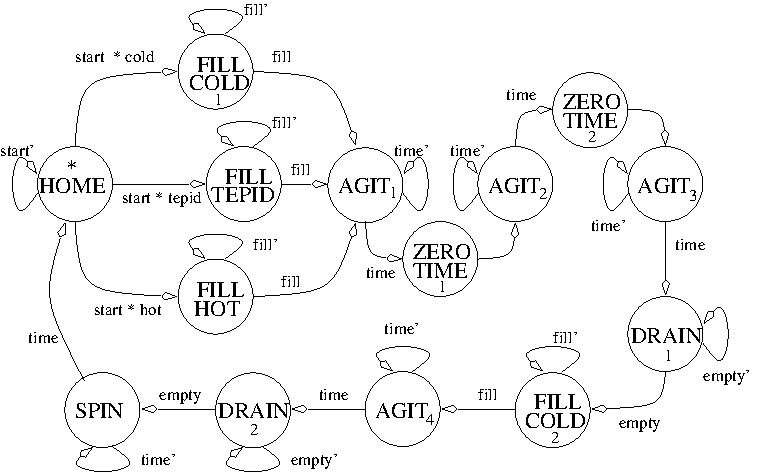
\includegraphics{Sol7-13}}
\caption{The FSM for a washing machine.}
\end{figure}

\begin{tabular}{|l|||l|l|l|l|l|} \hline
\multicolumn{6}{|c|}{outputs from the digital circuit}			\\ \hline \hline
state & hot     & cold    & motor      & timer in   & drain 	\\ \hline
      & 0 close & 0 close & 00 off     & 00 nothing & 0 close	\\ \hline
      & 1 open  & 1 open  & 01 agitate & 01 reset   & 1 open	\\ \hline
      &		&         & 10 spin    & 10 start   &		\\ \hline 
      &		&         &	       & 11 stop    &		\\ \hline \hline
HOME  &	0	& 0	  & 00	       & 00	    & 0		\\ \hline
COLD  &	0	& 1	  & 00	       & 01	    & 0		\\ \hline
TEPI  &	1	& 1	  & 00	       & 01	    & 0		\\ \hline
HOT   &	1	& 0	  & 00	       & 01	    & 0		\\ \hline
AGIT  &	0	& 0	  & 01	       & 10	    & 0		\\ \hline
ZERO  &	0	& 0	  & 00	       & 01	    & 0		\\ \hline
DRAI  &	0	& 0	  & 00	       & 01	    & 1		\\ \hline
SPIN  &	0	& 0	  & 10	       & 10	    & 0		\\ \hline
\end{tabular}

The memory input equations are a snap.  
\begin{description}
\item $D_{home} = Q_{home}start' + Q_{spin}time $
\item $D_{cold1} = Q_{home}*start*cold $
\item $D_{tepi} =  Q_{home}*start*tepid $
\item $D_{hot} =  Q_{home}*start*hot $
\item $D_{agit1} = Q_{cold1}*fill + Q_{tepid}*fill + Q_{hit}*fill + Q_{agit1}*time' $
\item $D_{zero1} =  Q_{agit1}*time $
\item $D_{agit2} = Q_{zero1}*time + Q_{agit2}*time' $
\item $D_{zero2} = Q_{agit2}*time $
\item $D_{agit3} = Q_{zero2}*time + Q_{agit2}*time' $
\item $D_{drain1} = Q_{agit3}*time + Q_{drain1}*empty' $
\item $D_{cold2} = Q_{drain1}*empty + Q_{cold2}*fill' $
\item $D_{agit4} =  Q_{cold2}*fill + Q_{agit4}*time' $
\item $D_{drain2} = Q_{agit4}*time + Q_{drain2}*empty' $
\item $D_{spin} = Q_{drain2}*empty + Q_{spin}*time' $
\end{description}

}\end{onlysolution} 


\item \textbf{ (36 pts.)}
Construct a digital circuit to control the movement of an elevator
in a four-story building.  The elevator will always wait on its current floor
until a call button is pressed; see Figure~\ref{fig:elevator}.  The elevator
then moves to the floor that was called.  The elevator then opens its doors and
waits for an elevator control button to be pressed.  If no elevator control
button is pressed and a call to another floor is received, then the elevator
closes the doors and goes to the new floor.  When a floor is selected on the
elevator control panel, then the door close and the elevator moves to the
desired floor.

\begin{figure}[ht]
\center{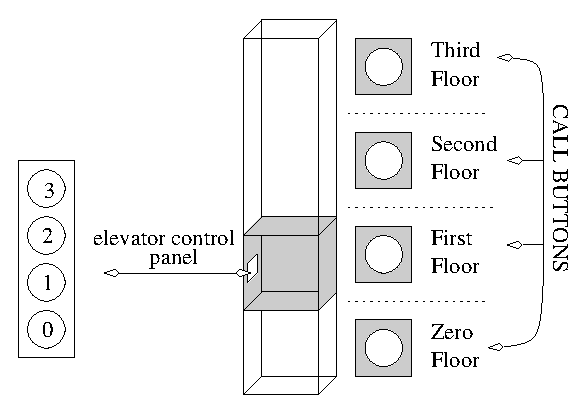
\includegraphics{Prob7-15}}
\caption{The layout of an elevator in a four story tall building.}
\label{fig:elevator}
\end{figure}

The inputs to the digital circuit clearly include all the buttons.
When a button is pressed on the elevators control panel two things
happen.  A 2-bit binary value representing the button pressed
becomes valid and a 1-bit panel request becomes valid.  The
panel request line will remain valid until acknowledged.

When a call button is pressed two things happen.  A 2-bit binary value
representing which call button was pressed becomes valid and a 1-bit
call request becomes valid.  The call request line will remain valid
until acknowledged.

Another input tells the circuit when the
elevator is or is not aligned with a floor.  For example, consider
an elevator moving from the first to the third floor.  Initially, the
align variable is 1.  When the elevator starts
to move away from the first floor towards the second, the align
variable goes to 0.  When the elevator reaches the second floor, the
align variable will go to logic 1 and remain there for a short
while (at least several milliseconds) because there is some
slack allowed in what is considered ``aligned".  After the elevator
passes the second floor, the align variable goes back to 0 and stays
there until the elevator reaches the third floor.

Here is the table of inputs to the FSM, their abbreviations, to be
used in the FSM, and their meaning.

\begin{tabular}{|l|l||l|l|} \hline
Control panel floor     & Pfloor        & 2-bit floor number & \\ \hline
Panel request           & Preq          & The panel has a valid floor & \\ \hline
Call floor              & Cfloor        & 2-bit floor number & \\ \hline
Call request            & Creq          & The call buttons have a valid floor & \\ \hline
Align                   & Align         & 0 not aligned & 1 Aligned \\ \hline
\end{tabular}

The outputs from the digital circuit to control the door and the
movement of the elevator.

\begin{tabular}{|l|l|l|l|} \hline
Panel acknowledge       & Pack  & Acknowledge the panel request & \\ \hline
Call acknowledge        & Cack  & Acknowledge the call request & \\ \hline
Door                    &  0 close &    1 open  &         \\ \hline
Motor                   &  00 stop &    01 up   & 10 down \\ \hline
\end{tabular}

Submit; an algorithm the datapath and control unit,
the control word table, the memory input equations, and output equations.

\item \textbf{ (36 pts.)}
Construct a digital circuit to control the movement of traffic
at the four way intersection shown in Figure~\ref{fig:crossroad}.

\begin{figure}[ht]
\center{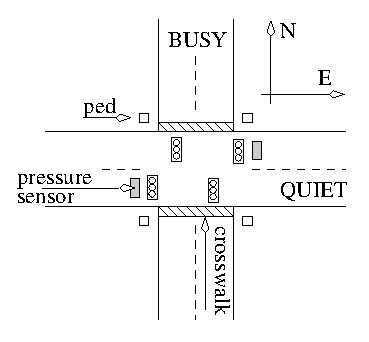
\includegraphics{Prob7-16}}
\caption{The layout of a four way intersection.}
\label{fig:crossroad}
\end{figure}

The circuit comes equipped with timers.
The timer has 2 inputs which set the timer to some preset
amount of time or allows the timer to count down.  When the
timer reaches 0 then the output of the timer goes to 1.
When the timer is not at 0 then the output equals 1.
The specific inputs and behavior are described in the following
truth table.

\begin{tabular}{|c|c|} \hline
timer input & behavior          \\ \hline \hline
00 & count down                 \\ \hline
01 & set to timer to 5  seconds \\ \hline
10 & set to timer to 15 seconds \\ \hline
11 & set to timer to 30 seconds \\ \hline
\end{tabular}

In addition to the timer there are a variety of real world inputs
sent to the circuit described in the following table.

\begin{tabular}{|l|l|l|} \hline
Name                    & Abbreviation & Function \\                       \hline \hline
E or W Pressure Sensor  & EW-PS & 1 if 250 lb. or more on E or W sensor \\ \hline
Ped button              & ped   & 1 if any pedestrian crosswalk button  \\ \hline
\end{tabular}

The outputs from the digital circuit to control the lights are:

\begin{tabular}{|l|l|l|l|} \hline
light           & 0x red &  10 yellow & 11 green \\ \hline
\end{tabular}

The main sequence of events is outlined below;
\begin{verbatim}
while(1) {
    Nlight = Slight = green;
    Elight = Wlight = red;
    wait 30 seconds;
    while ((EW-PS == 0) && (ped == 0));
    Nlight = Slight = yellow;
    wait 5 seconds;
    if (ped == 1) {
        Nlight = Slight = red;
        Elight = Wlight = red;
        wait 15 seconds;
    }
    Nlight = Slight = red;
    Elight = Wlight = green;
    wait 15 seconds;
    Elight = Wlight = yellow;
    wait 5 seconds;
    if (ped == 1) {
        Nlight = Slight = red;
        Elight = Wlight = red;
        wait 15 seconds;
}   }
\end{verbatim}


Submit;
the control unit,
the control word table,
the memory input equations, and
output equations.


\begin{onlysolution}  \textbf{Solution} \itshape{

\begin{figure}[ht]
\center{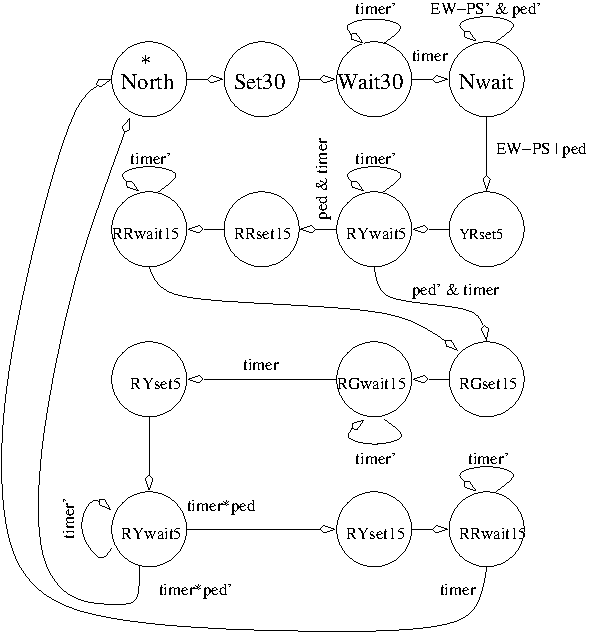
\includegraphics{Sol7-16}}
\caption{The FSM for a traffic light controller.}
\end{figure}

\begin{tabular}{|l|||l|l|l|} \hline
\multicolumn{4}{|c|}{outputs from the digital circuit}    \\ \hline \hline
state & Timer     & NS light  & EWlight     \\ \hline
      & 00 down   & 00 red    & 00 red      \\ \hline
      & 01 5 sec  & 01 red    & 01 red      \\ \hline
      & 10 15 sec & 10 yellow & 10 yellow   \\ \hline
      & 11 30 sec & 11 green  & 11 green    \\ \hline \hline
North	& 00 	  & 11	      & 00  \\ \hline
set30 & 11 	  & 11	      & 00  \\ \hline
wait30& 00 	  & 11	      & 00  \\ \hline
Nwait	& 00 	  & 11	      & 00  \\ \hline

YRset5  & 01 	  & 10	      & 00  \\ \hline
YRwait5 & 00 	  & 10	      & 00  \\ \hline

RRset15 & 10 	  & 00	      & 00  \\ \hline
RRwait15& 00 	  & 00	      & 00  \\ \hline

RGset15 & 10 	  & 00	      & 11  \\ \hline
RGwait15& 00 	  & 00	      & 11  \\ \hline
\end{tabular}


The memory input equations are a snap.
\begin{description}
\item $D_{North} = Q_{RYwait5}*ped*timer + Q_{RRwait15}*timer $
\item $D_{Set30} = Q_{North} $
\item $D_{Wait30} = Q_{Set30} + Q_{Wait30}*timer' $
\item $D_{Nwait} = Q_{Wait30}*timer + Nwait*EW_PS'*ped' $
\item $D_{YRset5} = Q_{Nwait}*(EW_PS + ped) $
\item $D_{YRwait5} = Q_{YRset5} +Q_{YRwait5}*timer' $
\item $D_{RRset15} = Q_{YRwait5}*ped*timer $
\item $D_{RRwait15} = Q_{RRset15} + Q_{RRwait15}*timer' $
\item $D_{RGset15} = Q_{YRwait5}*ped'*timer + Q_{RRwait15}*timer $
\item $D_{RGwait15} = Q_{RGset15} $
\item $D_{RYset5} = Q_{RGwait15}*timer' $
\item $D_{RYwait5} = Q_{RYset5} + Q_{RYwait5}*timer' $
\item $D_{RRset15} = Q_{RYwait5}*ped $
\item $D_{RRwait15} = Q_{RRset15} +Q_{RRwait15}*timer' $
\end{description}

The output equations
\begin{description}
\item $Z_{t1}  = Q_{set30} + Q_{RRset15} $
\item $Z_{t0}  = Q_{set30} + Q_{YRset5} $
\item $Z_{ns1} = Q_{North} + Q_{set30} + Q_{wait30} + Q_{Nwait} +Q_{YRset5}+Q_{YRwait5} $
\item $Z_{ns0} = Q_{North} + Q_{set30} + Q_{wait30} + Q_{Nwait} $
\item $Z_{ew1} = Q_{RGset15} + Q_{RGwait15} $
\item $Z_{ew0} = Q_{RGset15} + Q_{RGwait15} $
\end{description}
}\end{onlysolution} 
\end{enumerate}

